% Options for packages loaded elsewhere
\PassOptionsToPackage{unicode}{hyperref}
\PassOptionsToPackage{hyphens}{url}
%
\documentclass[
  english,
  man,mask,floatsintext]{apa7}
\usepackage{lmodern}
\usepackage{amssymb,amsmath}
\usepackage{ifxetex,ifluatex}
\ifnum 0\ifxetex 1\fi\ifluatex 1\fi=0 % if pdftex
  \usepackage[T1]{fontenc}
  \usepackage[utf8]{inputenc}
  \usepackage{textcomp} % provide euro and other symbols
\else % if luatex or xetex
  \usepackage{unicode-math}
  \defaultfontfeatures{Scale=MatchLowercase}
  \defaultfontfeatures[\rmfamily]{Ligatures=TeX,Scale=1}
\fi
% Use upquote if available, for straight quotes in verbatim environments
\IfFileExists{upquote.sty}{\usepackage{upquote}}{}
\IfFileExists{microtype.sty}{% use microtype if available
  \usepackage[]{microtype}
  \UseMicrotypeSet[protrusion]{basicmath} % disable protrusion for tt fonts
}{}
\makeatletter
\@ifundefined{KOMAClassName}{% if non-KOMA class
  \IfFileExists{parskip.sty}{%
    \usepackage{parskip}
  }{% else
    \setlength{\parindent}{0pt}
    \setlength{\parskip}{6pt plus 2pt minus 1pt}}
}{% if KOMA class
  \KOMAoptions{parskip=half}}
\makeatother
\usepackage{xcolor}
\IfFileExists{xurl.sty}{\usepackage{xurl}}{} % add URL line breaks if available
\IfFileExists{bookmark.sty}{\usepackage{bookmark}}{\usepackage{hyperref}}
\hypersetup{
  pdftitle={Modelling typing disfluencies using Bayesian mixture models},
  pdflang={en-EN},
  pdfkeywords={Copy-task; keystroke modelling; autoregression; mixture models; Bayesian statistical models; typing skills},
  hidelinks,
  pdfcreator={LaTeX via pandoc}}
\urlstyle{same} % disable monospaced font for URLs
\usepackage{graphicx}
\makeatletter
\def\maxwidth{\ifdim\Gin@nat@width>\linewidth\linewidth\else\Gin@nat@width\fi}
\def\maxheight{\ifdim\Gin@nat@height>\textheight\textheight\else\Gin@nat@height\fi}
\makeatother
% Scale images if necessary, so that they will not overflow the page
% margins by default, and it is still possible to overwrite the defaults
% using explicit options in \includegraphics[width, height, ...]{}
\setkeys{Gin}{width=\maxwidth,height=\maxheight,keepaspectratio}
% Set default figure placement to htbp
\makeatletter
\def\fps@figure{htbp}
\makeatother
\setlength{\emergencystretch}{3em} % prevent overfull lines
\providecommand{\tightlist}{%
  \setlength{\itemsep}{0pt}\setlength{\parskip}{0pt}}
\setcounter{secnumdepth}{-\maxdimen} % remove section numbering
% Make \paragraph and \subparagraph free-standing
\ifx\paragraph\undefined\else
  \let\oldparagraph\paragraph
  \renewcommand{\paragraph}[1]{\oldparagraph{#1}\mbox{}}
\fi
\ifx\subparagraph\undefined\else
  \let\oldsubparagraph\subparagraph
  \renewcommand{\subparagraph}[1]{\oldsubparagraph{#1}\mbox{}}
\fi
% Manuscript styling
\usepackage{upgreek}
\captionsetup{font=singlespacing,justification=justified}

% Table formatting
\usepackage{longtable}
\usepackage{lscape}
% \usepackage[counterclockwise]{rotating}   % Landscape page setup for large tables
\usepackage{multirow}		% Table styling
\usepackage{tabularx}		% Control Column width
\usepackage[flushleft]{threeparttable}	% Allows for three part tables with a specified notes section
\usepackage{threeparttablex}            % Lets threeparttable work with longtable

% Create new environments so endfloat can handle them
% \newenvironment{ltable}
%   {\begin{landscape}\begin{center}\begin{threeparttable}}
%   {\end{threeparttable}\end{center}\end{landscape}}
\newenvironment{lltable}{\begin{landscape}\begin{center}\begin{ThreePartTable}}{\end{ThreePartTable}\end{center}\end{landscape}}

% Enables adjusting longtable caption width to table width
% Solution found at http://golatex.de/longtable-mit-caption-so-breit-wie-die-tabelle-t15767.html
\makeatletter
\newcommand\LastLTentrywidth{1em}
\newlength\longtablewidth
\setlength{\longtablewidth}{1in}
\newcommand{\getlongtablewidth}{\begingroup \ifcsname LT@\roman{LT@tables}\endcsname \global\longtablewidth=0pt \renewcommand{\LT@entry}[2]{\global\advance\longtablewidth by ##2\relax\gdef\LastLTentrywidth{##2}}\@nameuse{LT@\roman{LT@tables}} \fi \endgroup}

% \setlength{\parindent}{0.5in}
% \setlength{\parskip}{0pt plus 0pt minus 0pt}

% \usepackage{etoolbox}
\makeatletter
\patchcmd{\HyOrg@maketitle}
  {\section{\normalfont\normalsize\abstractname}}
  {\section*{\normalfont\normalsize\abstractname}}
  {}{\typeout{Failed to patch abstract.}}
\makeatother
\shorttitle{Modelling typing disfluencies}
\author{Jens Roeser\textsuperscript{1}, Sven De Maeyer\textsuperscript{2}, Mariëlle Leijten\textsuperscript{3}, \& Luuk Van Waes\textsuperscript{3}}
\affiliation{
\vspace{0.5cm}
\textsuperscript{1} Department of Psychology, Nottingham Trent University, United Kingdom\\\textsuperscript{2} Faculty of Social Sciences, University of Antwerp, Belgium\\\textsuperscript{3} Department of Management, University of Antwerp, Belgium}
\authornote{

Correspondence concerning this article should be addressed to Jens Roeser, 50 Shakespeare St, Nottingham NG1 4FQ. E-mail: jens.roeser@ntu.ac.uk}
\keywords{Copy-task; keystroke modelling; autoregression; mixture models; Bayesian statistical models; typing skills}
\usepackage{csquotes}
\usepackage{booktabs}
\usepackage{longtable}
\usepackage{graphicx}
\usepackage{array}
\usepackage{multirow}
\usepackage{float}
\usepackage{colortbl}
\usepackage{threeparttable}
\usepackage[normalem]{ulem}
\usepackage[utf8]{inputenc}
\usepackage{icomma}
\usepackage{pdflscape}
\newcommand{\blandscape}{\begin{landscape}}
\newcommand{\elandscape}{\end{landscape}}
\ifxetex
  % Load polyglossia as late as possible: uses bidi with RTL langages (e.g. Hebrew, Arabic)
  \usepackage{polyglossia}
  \setmainlanguage[]{english}
\else
  \usepackage[shorthands=off,main=english]{babel}
\fi
\ifluatex
  \usepackage{selnolig}  % disable illegal ligatures
\fi
\newlength{\cslhangindent}
\setlength{\cslhangindent}{1.5em}
\newenvironment{cslreferences}%
  {\setlength{\parindent}{0pt}%
  \everypar{\setlength{\hangindent}{\cslhangindent}}\ignorespaces}%
  {\par}

\title{Modelling typing disfluencies using Bayesian mixture models}

\date{}

\abstract{
The analysis of keystroke-latency data typically involves the calculation of summary statistics such as the mean inter-keystroke interval and pause frequencies. There are two fundamental problems with this: first, summary statistics ignore important information in the data and frequently result in biased estimates; second, pauses and pause-related measures are defined using threshold values which are, in principle, arbitrary. We implemented a series of Bayesian models that aimed to address both issues by providing reliable estimates for individual typing speed and statistically inferred process disfluencies. We tested these models on a random sample of 250 copy-task recordings. Our results illustrate that we can model the copy typing as a mixture process of normal typing and typing disfluencies. We conclude that mixture models (1) map onto the information cascade that generate keystrokes, and (2) provide a principled approach to detect disfluencies in keyboard-typing data.
}

\begin{document}
\maketitle

\hypertarget{introduction}{%
\section{Introduction}\label{introduction}}

Writing research has made extensive use of keystroke-logging to capture typing-process data. In particular process disfluencies (loosely defined as relatively long intervals between subsequent keystrokes) are interesting to develop an understanding of an individual's writing dynamics. This is because language production is typically thought of as an information cascade from the mental generation of a message, into grammatical processing and finally the generation and execution of motor codes. This idea can be found in theoretical models of speech (Bock \& Ferreira, 2014), handwriting (Van Galen, 1991) and keyboard typing (Hayes, 2012). Disfluencies at the execution stage are therefore indicators of process demands that arise on higher levels of mental representation (Christiansen \& Chater, 2016; Olive, 2014); for example when preplanning syntactic dependencies (Roeser et al., 2019) or retrieving the lexical entry of a word or its spelling (Torrance et al., 2016). At present there is no principled way that allows us to detect lags at the execution stage that can be considered process disfluencies. In this paper we present a series of statistical models aiming to capture process disfluencies and produce by-participant estimates of typing performance.

Keystroke logs provide rich information about the typing process. From these log, researchers can calculate different process measures including measures of writing fluency (Chukharev-Hudilainen et al., 2019; Medimorec et al., 2017; Medimorec \& Risko, 2016; Van Waes \& Leijten, 2015). To name a few, researchers have performed data analysis on means, medians and standard deviations of inter-keystroke intervals (the latency between two consecutive keystrokes), number of pauses or pause duration and within-word keystroke intervals (for an overview of frequently used keystroke measures see Conijn, Roeser, et al., 2019). Conijn, Roeser, et al. (2019) suggested that these aggregates are sensitive to processing difficulty that arises on different levels of mental representation. However, there are two substantial problems tight to the use of summary statistics to develop an understanding of the typing process.

First, pause frequencies, writing bursts and related measures are used to assess writing performance (e.g.~Alves \& Limpo, 2015; Beers et al., 2017; Zhang et al., 2019). These measures require a definition of what passes as a pause (Van Waes et al., 2016; Wengelin, 2006), i.e.~a pause criterion threshold often set to 2 secs (Chanquoy et al., 1996; Kaufer et al., 1986; Sullivan \& Lindgren, 2002; Wengelin, 2002) or some other lower bounds (Chukharev-Khudilaynen, 2014; Connelly et al., 2012; Leijten \& Van Waes, 2013). Researchers have stipulated pause thresholds specific to their research purposes and based on prior research. However, ideally, this threshold would need to be specific to factors such as location in the text, writing task and the skills of the typist (Wengelin, 2006). For example, mid-word pauses require a different threshold than sentence-initial pausing. Also, when comparing the frequency of pauses larger than 2 secs for a dyslexic and a normal typist, one might observe more pauses for the dyslexic because 2 secs are indeed not unusual transitions between two keystrokes for a dyslexic writer and pauses for the normal typist are typically shorter than 2 secs and therefore unobserved given a 2-secs pause criterion (Wengelin, 2001). This bias would also affect the interpretation of results from L2 typists and other threshold criteria (Van Waes \& Leijten, 2015).

Second, data aggregation results in the loss of important information about disfluencies and time course variation. Even if this variation is not of interest to a research question, parametric aggregates such as mean and standard deviation, and even non-parametric descriptives such as median and interquartile range, are biased estimates for keystroke data. This is because many summary statistics, including the mean and the standard deviation, assume that the population, or process for writing data, that the data are sampled from is normally distributed. Keystroke intervals, however, are non-normally distributed; keystroke intervals are zero-bound and therefore right-skewed.\footnote{In fact, the minimum size of keystroke intervals is a function of the time it takes to plan and execute the motor program and keyboard polling.} Figure \ref{fig:example} illustrates this problem a sample taken from the copy-task log of two participants (from the copy-task data reported below). For the keystroke intervals of either participant, we contrast the density function of the empirical data (dashed line) and the normal density function (solid line). The normal density function is based on the observed mean (dotted vertical line) and standard deviation (see figure caption). Panel A shows the untransformed inter-keystroke intervals; Panel B shows the log-transformed data.

\begin{figure}[bp!]

{\centering 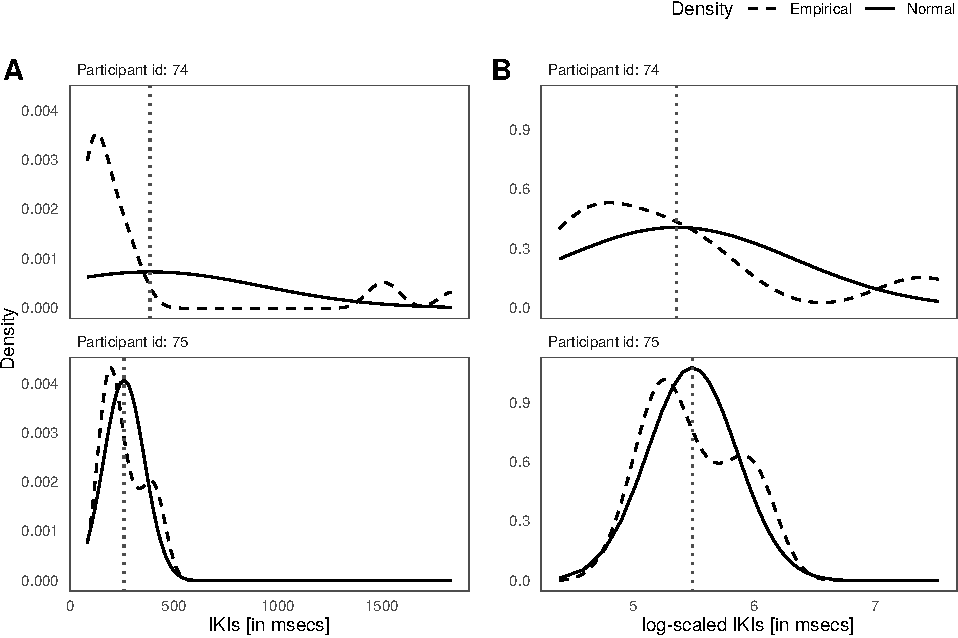
\includegraphics{report_files/figure-latex/example-1} 

}

\caption{Example for mean as biased estimator for the inter-keystroke intervals (IKIs) for two participants (participant 74 in the top panels; participant 75 in the bottom panels). All panels show the empirical density of the data and the normal-density function entailed by the observed mean (represented as dotted vertical line) and the standard deviation (SD): participant 74: mean=204 (SD=118), participant 75: mean=431 (SD=448). The untransformed IKIs are shown in plot A and the log-scaled IKIs are shown in plot B.}\label{fig:example}
\end{figure}

Importantly, Figure \ref{fig:example} shows that means of both the untransformed and the log-scaled keystroke data of participants 74 and 75 appear to be poor central-tendency estimates. This is evidenced by the mismatch between the observed data and the normal distribution entailed by the observed mean and standard deviation. This mismatch is not only due to the right skew in the keystroke data but might be related to a bimodal tendency that can be seen best in the log-scaled keystroke-intervals shown in Figure \ref{fig:example}B; the empirical-density function shows two peaks in both participants. The distribution of longer keystroke intervals is therefore going to influence any statistical quantity that assumes a normal distribution.

Therefore, data aggregation may lead to incorrect inference about the writing process (Baaijen \& Galbraith, 2018). To address biases in these estimates researchers have used data transformation, and data trimming (Hoaglin \& Iglewicz, 1987) to remove data that were \emph{a priori} considered outliers, or separated disfluencies (or pauses) from normal keystroke transitions. However log-transformation may account for positive skew but does not address the bimodality, as demonstrated in Figure \ref{fig:example}B. From existing research we know that keystroke data are not merely right-skewed, which can be addressed with log-normal transformations, but heavily right tailed (Almond et al., 2012; Baaijen et al., 2012; Chukharev-Khudilaynen, 2014; Guo et al., 2018). Further, using fixed threshold values to distinguish between normal and disfluent typing intervals will inevitably impact more on struggling writers (e.g.~participant 75) but also learners and and dyslexic individuals more generally) leading to larger data loss, less reliable typing estimates and therefore incorrect conclusions about the hypothesis tested. A pause threshold would need to be participant-specific (Wengelin, 2006) but is more difficult to determine for individuals with a larger variability (e.g.~participant 75 in Figure \ref{fig:example}A).

A central methodological challenge with implications for writing research (Hayes, 2012; Kaufer et al., 1986; Van Waes et al., 2016; Wengelin, 2006) is the detection of writing disfluencies. We addressed this problem by implementing statistical models that aim to capture the nature of the data generating cognitive process that underlies keyboard typing. Crucially we want a statistical model that provides reliable estimates of typing performance without subjecting the data to trimming or threshold criteria, aggregation or manual manipulation, and also accounts for typing disfluencies and other properties of the data (e.g.~individual typing style, key-pair specific differences).

\hypertarget{modelling-typing-process-data}{%
\section{Modelling typing process data}\label{modelling-typing-process-data}}

As a guiding principle, we aim to produce a statistical model that represents the mental process that generates the keystroke data. Keystrokes are the end of a cascade of mental processes. Lags between subsequent keypresses, for example, the transitions c\(^{\wedge}\)a\(^{\wedge}\)t for the word \emph{cat}, where \(^{\wedge}\) indicates the inter-keystroke intervals (IKI) between pressing \(<\)c\(>\) and \(<\)a\(>\), and \(<\)a\(>\) and \(<\)t\(>\), increase when the information flow into motor execution was interrupted on a higher level. Keystroke intervals reflect at minimum two states of this information flow: (1) either activation can flow into motor plans and keystroke transitions are normal; or (2) activation flow was inhibited on a level higher than the generation of a motor plan and therefore the keystroke transition increased.

For example, writing a word involves the retrieval of its name and, then, its spelling. If the writer knows both, activation can flow smoothly into the execution of the corresponding motor codes. However if the writer struggles to retrieve the spelling for or the lexical entry of a word, the activation flow is being interrupted. Inhibition is then resulting in process disfluencies expressed in a larger lag between adjacent keys. In copy-typing tasks we can constraint the underlying cognitive process by removing higher-level processes such as lexical planning and orthographic retrieval (Grabowski, 2008; Wallot \& Grabowski, 2013). Figure \ref{fig:model} illustrates a basic model of the copy-typing process (see also Yamaguchi \& Logan, 2014; Logan \& Crump, 2011; Salthouse, 1984). At the top level, some chunk of letters has to be visually encoded. The size of this chunk is to some extent specific to task, target string and individual typing skill / style. The visually encoded sequence has to be buffered and, then, corresponding motor codes have to be activated. If there are no more motor codes that can be generated from the buffered information, visual encoding is required to update the buffer.

\begin{figure}[bp!]

{\centering 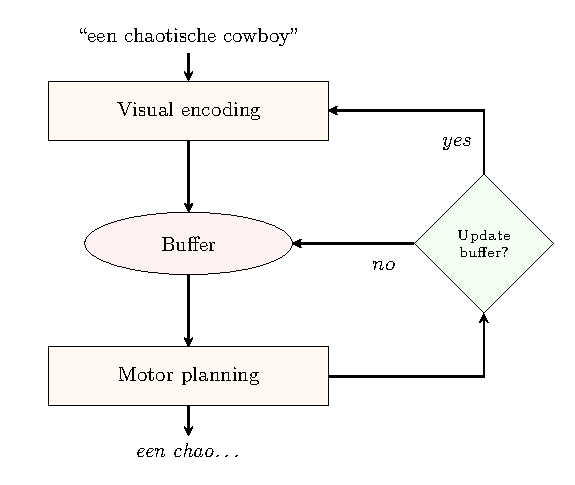
\includegraphics{spelling_decision} 

}

\caption{Basic model of copy typing; example for ``een chaotische cowboy'' (a chaotic cowboy).}\label{fig:model}
\end{figure}

The consequence of buffer updates is a slowdown in keystroke intervals (i.e.~a pause, disfluency) that cannot be explained on the basis of lexical retrieval or difficulty with particular bigrams. Figure \ref{fig:example2} shows the by-bigram IKIs of three participants copy-typing the (Dutch equivalent of the) phrase \emph{a chaotic cowboy}. These example data illustrate that disfluencies are not bigram-related difficulty. Participant 240 shows a small disfluency between \(<\)c\(>\) and \(<\)h\(>\) but no other notable slowdown; participant 105 shows a large disfluency between \(<\)o\(>\) and \(<\)t\(>\); participant 238 shows three disfluencies in total. Importantly, although to-be-copied words were the same, the number, location, and size of the disfluency/ies varied across participants. The model in Figure \ref{fig:model} explains these disfluencies as buffer updates. Our statistical model should provide a systematic way of addressing process disfluencies, even though their occurrence is, to some extent, non-deterministic (i.e.~can not be predicted on the basis of letter identity or bigram location).

\begin{figure}[bp!]

{\centering 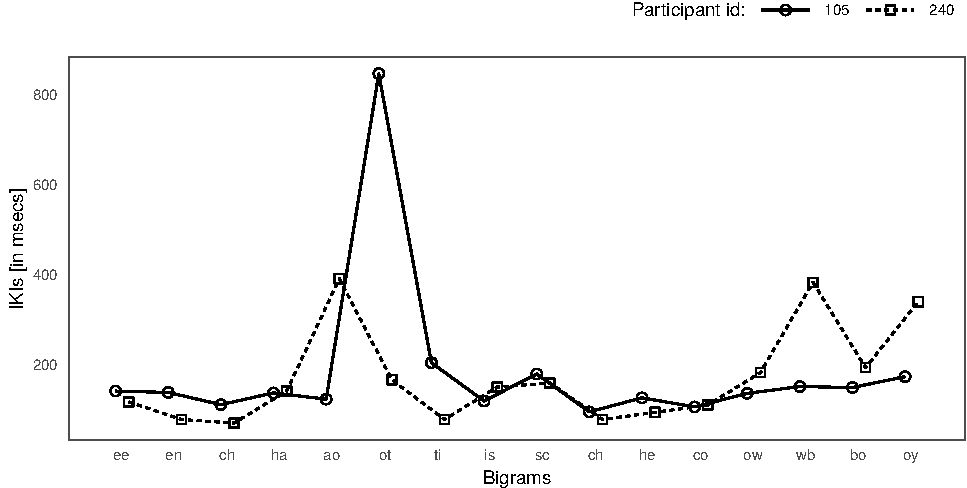
\includegraphics{report_files/figure-latex/example2-1} 

}

\caption{Example of the inter-keystroke intervals (IKIs) from three participants, shown as different linetypes, copy-typing ``een chaotische cowboy'' (a chaotic cowboy).}\label{fig:example2}
\end{figure}

Statistical models can be used to characterize the underlying data-generating process as a function of parameters. For example, if we assume that there is a single underlying process that generates normal distributed data, we can describe this process with a mean \(\mu\) and a variance \(\sigma^2\). The values of the parameters \(\mu\) and \(\sigma^2\) are unknown and typically used to represent and compare task and population specific (typing) performance. The model of the data can be written as \(y \sim Normal(\mu, \sigma^2)\); i.e.~the data \(y\) come from a single process that follows a normal distribution with an unknown mean \(\mu\) and an error variance \(\sigma^2\). We can then feed data to our statistical model to determine values for its parameters. The resulting parameter estimates can be considered reliable if the data-generating (cognitive) process matches the process assumed by the model; i.e.~the data come from a single process that generates normal distributed data.

\hypertarget{log-normal-mixed-effects-model-of-typing}{%
\subsection{Log-normal mixed-effects model of typing}\label{log-normal-mixed-effects-model-of-typing}}

For the first model, the baseline model, we will assume that IKIs follow a log-normal distribution (e.g.~Almond et al., 2012; Guo et al., 2018) because IKIs are zero-bound and therefore right skewed (Baayen, 2008).\footnote{We discussed above that the heavy tail associated with keystroke data is not necessarily fitting a log-normal distribution. We used this model as it is roughly equivalent to the standard statistical method used in the field (e.g.~fitting parametric models to log-transformed data).} This model is characterising the information cascade that generates keystroke intervals with the population mean \(\mu\).

To estimate the mean \(\mu\) we need to be able to account for variability that is caused by factors related to the sampling process. This can be achieved with log-normal (linear) mixed-effects models (LMM) which have been used in the literature to model keystroke data (Leijten et al., 2011; Quené \& Van den Bergh, 2004; Van Waes et al., 2010, 2020). The LMM in equation \ref{eq:lmm} is an extension of the simple example above. We know that some participants are faster typists than other participants and some bigrams are easier to type than others. Writers vary generally in how fast they type, or how quickly they are performing in the given task. Further more frequent bigrams (as part of words with a large number of occurrences in a corpus or bigrams that occur in many different words) are typically typed faster than low frequency bigrams; bigrams that are part of words are typed faster than novel bigrams; bigrams within morphological boundaries are typed faster than bigrams that cross morphological boundaries (Feldman et al., 2019; Nottbusch et al., 2005; Pinet et al., 2016; Sahel et al., 2008). In other words, IKIs for participants and bigrams are varying around a common mean. These sources of random-error variance are captured by \(u\) for participants and \(w\) for keystroke bigrams in equation \ref{eq:lmm}.

\[
\tag{1}
\begin{aligned}
y_{ij} \sim LogNormal(\mu + u_i + w_j, \sigma_e^2)\\
\end{aligned}
\label{eq:lmm}
\]

Differences associated with participant \(i\), expressed as \(u_i\), can be assumed to be normally distributed around 0 with a between-participants variance \(\sigma_u^2\) with \(i = 1, \dots, I\), where \(I\) is the number of participants (see \ref{eq:lmm2}). We can assume that this variance of \(\sigma_u^2\) is normally distributed, but because is a variance it can not ever be negative. We therefore assume a normal distribution, cut off at zero, and choose 2.5 as the variance, because the majority of participants should have, by definition, an average IKI close to zero with fewer participants being much faster or slower than the average. A variance of 2.5 is a reasonably informative prior that ensures that the variability across participants is approximately normal. This type of distribution is known as a half-normal (Gelman, 2006).

\[
\tag{2}
\begin{aligned}
u_i \sim Normal(0,\sigma_u^2)\\
\sigma_u \sim Normal(0,2.5)\\
\text{constraint: } \sigma_u >0 
\end{aligned}
\label{eq:lmm2}
\]

Similar to variability between participants we can model variation between keystroke pairs (i.e.~letter bigrams) as random-intercepts term; \(w\) in equation \ref{eq:lmm} (Van Waes et al., 2019; Van Waes et al., 2020). More specifically, this is to assume that each bigram \(j\) with \(j = 1, \dots, J\), where \(J\) is the total number of bigrams, is independent of the other bigrams. Each bigram-intercept difference \(w_j\) is distributed around 0 with a between-bigram variance \(\sigma_w^2\) (equation \ref{eq:lmm5}).

\[
\tag{3}
\begin{aligned}
w_j \sim Normal(0,\sigma_w^2)\\
\sigma_w \sim Normal(0,2.5)\\
\text{constraint: }\sigma_w >0 
\end{aligned}
\label{eq:lmm5}
\]

The parameter of interest, the mean \(\mu\) in equation \ref{eq:lmm}, is the marginalised value after taking into account random variation between participants and bigrams. In all models we parameterised the mean \(\mu\) as non-centered with regulating priors (equation \ref{eq:lmm3}; following Gelman et al., 2014; Papaspiliopoulos et al., 2007). Non-centering parameters can be used to aid sampling efficiency of the model. In other words, a more reliable parameter estimate can be achieved with the same number of iterations. For the mean \(\alpha_\mu\) of the population mean \(\mu\), we proposed a normal distributed prior centered around 5 (i.e.~log of \(\approx\) 150 msecs).

\[
\tag{4}
\begin{aligned}
\mu = \alpha_{\mu} + \sigma_{\mu} \cdot \epsilon\\
\alpha_{\mu} \sim Normal(5,2)\\
\sigma_{\mu} \sim Normal(0,1)\\
\epsilon \sim Normal(0,1)\\
\text{constraint: }\mu_{\sigma}>0 
\end{aligned}
\label{eq:lmm3}
\]

For the unexplained residual variance \(\sigma_e^2\), we used an uninformative half-Cauchy prior (equation \ref{eq:lmm4}; as mentioned in Gelman et al., 2014). The Cauchy is a heavy tailed distribution; a centre of 0 indicates that the residual variance should be close to 0 but the scale 2.5 allows for larger values.

\[
\tag{5}
\begin{aligned}
\sigma_e \sim Cauchy(0,2.5)\\
\text{constraint: }\sigma_e>0 
\end{aligned}
\label{eq:lmm4}
\]

\hypertarget{typing-as-autoregressive-process}{%
\subsection{Typing as autoregressive process}\label{typing-as-autoregressive-process}}

The previous model captures variation associated with bigrams but assumes that their locations are independent and thus exchangeable. In other words, keystroke intervals depend on the identity of the associated bigram but not on the duration of a preceding keystroke interval. There is however evidence that keystroke intervals tend to be longer at certain locations, before phrases (Roeser et al., 2019), words (Torrance et al., 2016), and on morphological boundaries (Nottbusch et al., 2005), and keystroke intervals tend to be shorter within words. IKIs are not necessarily independent of preceding keystroke intervals; an IKI \(y_{i}\) might be related to the IKI \(y_{i-1}\) preceding it, for example, such that a disfluency impacts on neighbouring keystroke intervals (Conijn, Van Zaanen, et al., 2019). The relationship between subsequent keystrokes can be captured by predicting an IKI with the IKI preceding it. This is called an autoregressive process (Eltahir et al., 2004); in equation \ref{eq:ark} the relationship between subsequent IKIs is captured by the parameter \(\phi\). As the degree of autocorrelation might vary with typing skill, we assumed that the autocorrelation varies between participants \(\phi_i\) with a centered mean \(\mu_{\phi}\) and error variance \(\eta^2\).

\[
\tag{6}
\begin{aligned}
y_{ij} \sim LogNormal(\mu + \phi_i \cdot log(y_{ij-1}) + u_i + w_j, \sigma_e^2)\\
\text{where}\\
\phi_i \sim Normal(\mu_{\phi}, \eta^2)\\
\mu_{\phi} \sim Normal(0, 1)\\
\eta \sim Cauchy(0, 1)\\
\text{constraint: }\eta >0 
\end{aligned}
\label{eq:ark}
\]

\hypertarget{typing-as-mixture-process}{%
\subsection{Typing as mixture process}\label{typing-as-mixture-process}}

So far we constructed models that account for the keystroke-interval differences associated with different typists, bigrams and that accounts for autocorrelation between subsequent keystroke-intervals. Next we will add a modelling component that allows us to distinguish between fluent and disfluent keystroke intervals using what is called a finite mixture-process model.

Mixture models are a straight-forwarded way of representing a data-generating process that involves a combination of different subprocesses (e.g.~Farrell \& Lewandowsky, 2018; Gelman et al., 2014). Finite-mixture models have been used to represent cognitive processes in which larger values arise in a probabilistic manner (see e.g.~Vasishth et al., 2017; Vasishth et al., 2017). Keystroke disfluencies in writing can be represented in a similar way. For keystroke data, the assumed process is a finite mixture (i.e.~combination) of two processes representing (1) normal typing, when activation can flow from higher into lower mental levels, and (2) typing disfluencies, when activation flow is interrupted (e.g.~for a buffer update). In other words, we fixed the number of underlying distributions to two, namely 2 log-Gaussian (log-normal) distributions, of which one represents fluent typing (shorter IKIs) and the other represents disfluencies (longer IKIs).

This model can be summarised as in equation \ref{eq:mog}, following Vasishth et al. (2017). The first and second line express that the data \(y\) are modelled as the sum of two weighted log-normal distributions of which the first distribution has a mixing proportion \(\theta\) (weight) and the other distribution receives the remaining proportion \(1-\theta\). \(\theta\) was used here as the unknown probability of process disfluencies. This was achieved by fixing the mean \(\mu\) for both distributions but adding the parameter \(\delta\), that was constrained to be positive, to the first distribution. \(\delta\) is therefore capturing the latency magnitude of process disfluencies with \(\theta\) indicating the probability of disfluencies to occur. The probability of disfluent IKIs was allowed to vary across participants \(i\) and stored in \(\theta_i\). This is because the probability to exhibit disfluencies can be assumed to depend on individual typing style (and skills).

\[
\tag{7}
\begin{aligned}
    y_{ij} \sim \theta_i \cdot LogNormal(\mu + \delta + u_i + w_j, \sigma_{e'}^2) +\\
        (1 - \theta_i) \cdot LogNormal(\mu + u_i + w_j, \sigma_{e}^2)\\
        \text{where}\\
        \delta \sim Normal(0,1)\\
        \text{constraint: } \delta > 0
\end{aligned}   
\label{eq:mog}
\]

To increase sampling efficiency we placed a continuous prior on the logit of the individual mixing proportions \(\alpha_i\), which was transformed to range between 0 and 1, using the inverse-logit function, and stored in \(\theta_i\). This is shown in equation \ref{eq:mog2}. We used a normal prior for the logit of individual mixing proportions \(\alpha_i\) with a mean \(\mu_{\alpha}\) that captures the logit of the population disfluency-probability (with an error variance \(\tau^2\)). The hyper-prior on the population mixing-proportion \(\mu_{\alpha}\) was assumed to have a mean of logit 0, corresponding to a probability of 0.5 and a variance of logit 1 (i.e.~\(\approx\) 0.73 in proportions).

\[
\tag{8}
\begin{aligned}
        \theta_i = Logit^{-1}(\alpha_i)\\
        \alpha_i \sim Normal(\mu_{\alpha},\tau^2)\\
        \mu_{\alpha} \sim Normal(0,1)\\
        \tau \sim Cauchy(0,1)\\
        \text{constraint: } \tau > 0
\end{aligned}   
\label{eq:mog2}
\]

As longer latencies are known to be associated with a larger variances for both response-time data in particular (Wagenmakers \& Brown, 2007) and human motor behaviour in general (Schöner, 2002; Wing \& Kristofferson, 1973), we constrained the variance \(\sigma_{e'}^2\) associated with the distribution of typing disfluencies to be larger than the variance for normal typing \(\sigma_e^2\); see equation \ref{eq:mog3} (see Vasishth et al., 2017; Vasishth et al., 2017).

\[
\tag{9}
\begin{aligned}
        \sigma_{e'} = \sigma + \sigma_{\text{diff}}\\
        \sigma_{e} = \sigma - \sigma_{\text{diff}}\\
        \sigma_{\text{diff}} \sim Normal(0,1)\\
        \sigma \sim Cauchy(0,2.5)\\
        \text{constraint: } \sigma, \sigma_{\text{diff}}, \sigma_{e'}, \sigma_{e} > 0
\end{aligned}   
\label{eq:mog3}
\]

\hypertarget{typing-as-autoregressive-mixture-process}{%
\subsection{Typing as autoregressive mixture process}\label{typing-as-autoregressive-mixture-process}}

The mixture model, as well as the LMM, assume that lags between subsequent letter bigrams are independent of each other; the argument against this was introduced above for autoregressive models. We implemented another mixture model that is largely equivalent to the model presented in the previous section but includes an autoregressor as in equation \ref{eq:ark}; see equation \ref{eq:mogark} for the autoregressive mixture-process model.

\[
\tag{8}
\begin{aligned}
    y_{ij} \sim \theta_i \cdot LogNormal(\mu + \delta + \phi_i \cdot log(y_{ij-1}) + u_i + w_j, \sigma_{e'}^2) +\\
        (1 - \theta_i) \cdot LogNormal(\mu + \phi_i \cdot log(y_{ij-1}) + u_i + w_j, \sigma_{e}^2)\\
\end{aligned}   
\label{eq:mogark}
\]

\hypertarget{method}{%
\section{Method}\label{method}}

To test which model captures the typing process best, we applied the four models described in the previous section to data from a subset of the Dutch copy-task corpus (Leijten \& Van Waes, 2013; Van Waes et al., 2019; Van Waes et al., 2020). An overview of all models can be found in Table \ref{tab:models}.

\begin{table}[bp!]

\begin{center}
\begin{threeparttable}

\caption{\label{tab:models}Overview of typing-process models. All models were fitted with random intercepts for participants and bigrams.}

\begin{tabular}{llll}
\toprule
Models & \multicolumn{1}{c}{Type} & \multicolumn{1}{c}{Equation} & \multicolumn{1}{c}{Description}\\
\midrule
M1 & LMM & \ref{eq:lmm} & Baseline model\\
M2 & AR & \ref{eq:ark} & Autocorrelation between subsequent IKIs\\
M3 & MoG & \ref{eq:mog} & Mixture process of fluent and disfluent typing\\
M4 & AR + MoG & \ref{eq:mogark} & As M3 but with autocorrelation component\\
\bottomrule
\addlinespace
\end{tabular}

\begin{tablenotes}[para]
\normalsize{\textit{Note.} LMM = Linear mixed-effects models; AR = Autoregressive model; MoG = Mixture of log-Gaussians}
\end{tablenotes}

\end{threeparttable}
\end{center}

\end{table}

The copy-task corpus consists of keystroke data collected via Inputlog, a Javascript-based web application available on \url{www.inputlog.net} with the source code released on \href{https://github.com/lvanwaes/Inputlog-Copy-Task}{github.com/lvanwaes/Inputlog-Copy-Task} and \href{https://zenodo.org/record/2908966}{zenodo.org/record/2908966}. In a set of different subtasks participants had to produce keyboard-typed responses. We used a random sample of 250 participants (178 females, 69 males, 3 unknown) from the age range of 18 to 25 years (median age = 22 years). Before analysis we excluded spaces and editing operations from the data.

In this analysis we focus on the consonants task and the low-frequency (LF) bigrams task. In the consonants task, participants saw and copy-typed a single time four blocks of six consonants; i.e.~\enquote{tjxgfl pgkfkq dtdrgt npwdvf}. This task is intended to measure typing skills in a non-lexical environment (Grabowski et al., 2010). We repeated the analysis for the LF-bigrams task to contrast the non-lexical consonants task and a lexical copy task. In the LF-bigram task, participants typed three-word combinations seven times (\emph{een chaotische cowboy} \enquote*{a chaotic cowboy} in the Dutch version) of which four bigrams are low frequent.\footnote{Note, we refer to this task as \emph{LF}-bigrams task as in Van Waes et al. (2019). The majority of bigrams in the target-word group is highly frequent.} For comparability to the consonants task, we removed all repetitions after the first time the three-word sequence was copied.

Importantly for the present purpose, fluent copying and pausing may be thought of as a function of (1) the familiarity with the letter sequences and (2) the participant's memory span and typing skill; for example touch-typists may depend less on memory representation of the to-be typed bigrams for fluent copying than hunt-and-peck typists. This results in a combination of fluent typing and typing interruptions. In other words, for these tasks we need to be able to disentangle fluent and disfluent IKIs.

Bayesian models, as used in this paper, are ideal for the reliable estimation of parameter values expressed as probability distribution rather than point estimates (Farrell \& Lewandowsky, 2018; Gelman et al., 2014; Lee \& Wagenmakers, 2014). To achieve this, Bayesian models require the explicit inclusion of prior information, i.e.~existing knowledge about parameter values. For small data sets non-uninformative priors influence the inferred parameter estimates (known as posterior) but for larger data sets vague priors are quickly overcome by the data (i.e.~automatic Ockam's razor; Jefferys \& Berger, 1992) so that the choice of priors values impacts the posterior to a lesser extent. In the present paper, priors are used to aid model convergence by constraining the parameter space (i.e.~using weakly regulating priors; Lambert, 2018; McElreath, 2016). Priors are described in the modelling section. The predictive performance (i.e.~fit) of these models is compared in the Results section.

\hypertarget{results}{%
\section{Results}\label{results}}

\hypertarget{data-overview}{%
\subsection{Data overview}\label{data-overview}}

The IKI data for the LF-bigrams task and the consonants task are visualized in Figure \ref{fig:descriptives}. The upper panels of the LF-bigrams task and the consonants task in Figure \ref{fig:descriptives}A show the data for each participant. In the lower panels of Figure \ref{fig:descriptives}A, different measures of central tendency are shown. The density function of the IKI data are shown in Figure \ref{fig:descriptives}B with vertical lines corresponding to the central tendency measures in Figure \ref{fig:descriptives}A.

\begin{landscape}
\begin{figure}[bp!]

{\centering 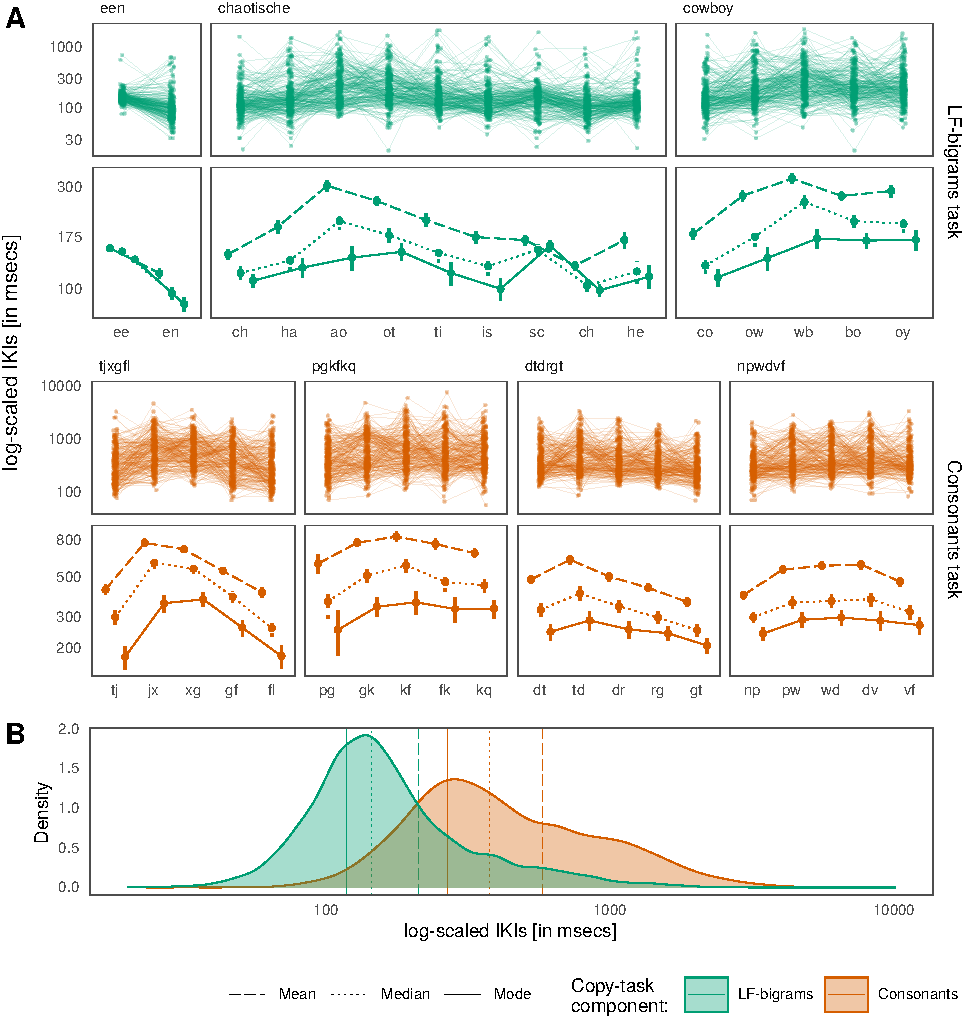
\includegraphics{report_files/figure-latex/descriptives-1} 

}

\caption{Data overview. Plot A illustrates IKIs over bigram position (time-course) by participant in the upper rows and as different measures of central tendency (with standard error [SE]) in the lower rows for each the LF-bigrams task and the consonants task. Plot B shows the density distribution of IKI data with the same central-tendency descriptors as in plot A.}\label{fig:descriptives}
\end{figure}
\end{landscape}

These visualisation highlight two important points for the present data that were discussed in the introduction section: (1) aggregating data neglects individual time-course variability in the data; (2) the choice of central-tendency measure leads to different conclusions about the data. As for the first point, Figure \ref{fig:descriptives}A shows that participants slowdowns and speedups throughout the trial but do not show consistent patterns for the same letter bigrams as might be concluded from the corresponding summary statistics. If we disregard by-participant variability, central-tendency measures in the lower panels of Figure \ref{fig:descriptives}A suggest that some slowdowns and speedups might be bigram specific. For example, in the LF-bigrams task, the first bigram is followed by a faster IKI; in the consonants task, the first bigram is followed by a slowdown. Importantly though, there is a substantial variability between participants.

As for the second point, the choice of central-tendency measure might affect whether we consider an observation a disfluency, or a participant to be prone to disfluent typing. In particular, means are systematically longer than the median and mode. Figure \ref{fig:descriptives}B illustrates why this is the case. Shown are the density functions for the LF-bigrams and the consonants task. Even log-scaled data show skewed distributions with a heavy right tail. While in a normal distribution the mean, median and mode have identical values, the conceptual differences between these three measures of central tendency lead to different values in non-normal distributed data. In particular, means are known to be sensitive to extreme values; these are inevitable for zero-bound IKIs with, in principle, no upper bound. For keystroke data, large means might be the consequence of a few larger IKIs that over-shadow largely normal typing behaviour. Means are closer to the horizontal middle of the data space which, for right-skewed distributions, is on the right of the distribution's peak (the value with the highest kernel density). The latter is being represented by the mode. Regardless of which measure is used, all three central tendency indicators ignore important properties of the distribution. That is, measures of central tendency neglect the variability in the data; keystroke data might indeed represent a combination of processes; e.g.~normal typing and disfluencies. Central tendency measures do not allow us to distinguish between IKIs that are the results of fluent typing and IKIs that reflect process lags.

For our data, aggregation does not just neglect participant-specific typing patterns but the choice of central-tendency measure leads to different conclusions about the data (e.g.~which IKIs can be considered pauses). To ensure accurate statistical inference, we need to be able to account for participant-specific typing patterns as expressed across the typing time-course.

\hypertarget{model-fit}{%
\subsection{Model fit}\label{model-fit}}

All models were implemented as Bayesian models (see e.g.~Gelman et al., 2014; Lambert, 2018; McElreath, 2016) in the probabilistic programming language Stan (Carpenter et al., 2016; Hoffman \& Gelman, 2014; Stan Development Team, 2015a, 2015b). Data, R-scripts and Stan-code are available on OSF (\href{https://osf.io/y3p4d/?view_only=2fe3472b599e4b53a17c461f44969aae}{osf.io/y3p4d/?view\_only=2fe3472b599e4b53a17c461f44969aae})\footnote{Anonymised clickable link for blind peer review.}. Models were fitted with 30,000 iterations (15,000 warm-up) on 3 MCMC chains. Convergence was tested via the Rubin-Gelman statistic (Gelman \& Rubin, 1992), traceplots and cross-validation (Vehtari et al., 2015, 2017).

The predictive performance of the models was established using leave-one-out cross-validation. Cross-validation penalizes models with more parameters and therefore prevents overfit (see Farrell \& Lewandowsky, 2018; Lambert, 2018; Lee \& Wagenmakers, 2014; McElreath, 2016). The out-of-sample predictive performance was determined via Pareto smoothed importance-sampling (Vehtari et al., 2015, 2017) and estimated as sum of the expected log predictive density (\(\widehat{elpd}\)). \(\widehat{elpd}\) was used to compare the predictive quality of our models. Model comparisons can be found in Table \ref{tab:modelcomparisons}. Model comparisons revealed higher predictive performance for both mixture models M3 and M4 for both copy-task components. The increase in predictive performance is larger for the LF bigrams task compared to the consonants task. The differences in predictive performance of all models shows the same pattern in both copy-task components. For both tasks, the combination of the mixture model and the autoregressive-process model as implemented in model M4 (see equation \ref{eq:mog}) revealed the highest predictive performance with a small advantage over mixture model M3 (see equation \ref{eq:mogark}). We therefore chose model M4 for parameter evaluation of both copy-task components.

\begin{table}[bp!]

\begin{center}
\begin{threeparttable}

\caption{\label{tab:modelcomparisons}Model comparisons expressed as expected log predictive density ($\widehat{elpd}$). The top row of each copy-task component shows the model with the highest predictive performance. Differences in predictive performance are shown as $\Delta\widehat{elpd}$ contrasting for each copy-task component the model in the first row and the remaining models. Standard errors (SE) are shown in brackets.}

\begin{tabular}{lllr}
\toprule
Model & \multicolumn{1}{c}{Type} & \multicolumn{1}{c}{$\Delta\widehat{elpd}$} & \multicolumn{1}{c}{$\widehat{elpd}$}\\
\midrule
Consonants &  &  & \\
\ \ \ M4 & AR + MoG & 0 (0) & -37,032 (102)\\
\ \ \ M3 & MoG & -38 (7) & -37,069 (101)\\
\ \ \ M2 & AR & -264 (25) & -37,295 (100)\\
\ \ \ M1 & LMM & -318 (25) & -37,350 (99)\\
LF bigrams &  &  & \\
\ \ \ M4 & AR + MoG & 0 (0) & -33,148 (113)\\
\ \ \ M3 & MoG & -30 (8) & -33,178 (113)\\
\ \ \ M2 & AR & -1,011 (64) & -34,159 (121)\\
\ \ \ M1 & LMM & -1,025 (64) & -34,173 (121)\\
\bottomrule
\addlinespace
\end{tabular}

\begin{tablenotes}[para]
\normalsize{\textit{Note.} LMM = Linear mixed-effects models; AR = Autoregressive model; MoG = Mixture of log-Gaussians}
\end{tablenotes}

\end{threeparttable}
\end{center}

\end{table}

\hypertarget{parameter-evaluation}{%
\subsection{Parameter evaluation}\label{parameter-evaluation}}

The copy-typing process can be characterized by the posterior of the mixture model's parameter values. These parameters values are summarised in Table \ref{tab:modelparameters} and in Figure \ref{fig:parameters}. Table \ref{tab:modelparameters} summarises the population and variance estimates as posterior mean with 95\% probability intervals (PI). Estimates are shown for the LF-bigrams task and the consonants task. After accounting for process disfluencies, keystroke intervals were longer for the consonants task (429 msecs, PI {[}356, 515{]}) compared to the LF-bigrams task (158 msecs, PI {[}139, 180{]}). The slowdown for disfluencies was about four times longer for the consonants task. For the LF-bigrams task, the model determined a slowdown of 95 msecs (PI {[}76, 116{]}) with a probability of 0.34 (PI {[}0.31, 0.38{]}); for the consonants task we found a slowdown of 414 msecs (PI {[}333, 509{]}) with a probability of 0.73 (PI {[}0.66, 0.80{]}). In other words, in the consonants disfluent keystroke transitions were three times more likely to occur than fluent transitions; in the LF-bigrams task, only one out of three transitions constitutes a disfluency. The size of the slowdown in the consonants task suggest higher level processes such as reading of the target string. This is unlikely to be the case for the short slowdown in the LF-bigrams task. Instead, the slowdown in the LF-bigrams task might be a bigram-frequency effect. Four out of 16 bigrams in the LF-bigrams have a low frequency (i.e.~\(\frac{4}{16}\approx0.19\)). In other words, the magnitude for disfluencies and hence their cognitive source in the typing process is task-specific. Further autocorrelation between subsequent keystrokes was non-different from zero in the LF-bigrams task; keystroke transitions in the consonants task were in general followed by a -0.08 times faster keystroke transition; PI {[}-0.10, -0.05{]}. Variance components are reported for completeness.

\begin{table}[bp!]

\begin{center}
\begin{threeparttable}

\caption{\label{tab:modelparameters}Parameter estimates with 95\% PIs separated into population estimates and estimates for variance components. Parameters are shown as used in equations with a brief description of their conceptual meaning in parentheses. Estimates are shown for the LF-bigrams task and the consonants task.}

\begin{tabular}{lrr}
\toprule
Parameter & \multicolumn{1}{c}{LF bigrams} & \multicolumn{1}{c}{Consonants}\\
\midrule
Population estimates &  & \\
\ \ \ $\beta$ (fluent typing) & 158 [139, 180] & 429 [356, 515]\\
\ \ \ $\delta$ (disfluency slowdown) & 95 [76, 116] & 414 [333, 509]\\
\ \ \ $\theta$ (disfluency probability) & 0.34 [0.31, 0.38] & 0.73 [0.66, 0.8]\\
\ \ \ $\phi$ (autoregressor) & 0 [-0.02, 0.02] & -0.08 [-0.1, -0.05]\\
Variance estimates &  & \\
\ \ \ $\sigma^2$ (residual error) & 0.73 [0.7, 0.75] & 0.54 [0.52, 0.56]\\
\ \ \ $\sigma_e^2$ (fluent typing) & 0.29 [0.27, 0.3] & 0.29 [0.26, 0.32]\\
\ \ \ $\sigma_{e'}^2$ (disfluency) & 1.16 [1.12, 1.21] & 0.79 [0.77, 0.81]\\
\ \ \ $\eta^2$ (autoregressor) & 0.04 [0.04, 0.05] & 0.01 [0, 0.02]\\
\ \ \ $\sigma_u^2$ (between-participants) & 0.03 [0, 0.08] & 0.27 [0.23, 0.31]\\
\ \ \ $\sigma_w^2$ (between-bigrams) & 0.22 [0.17, 0.3] & 0.24 [0.17, 0.33]\\
\bottomrule
\end{tabular}

\end{threeparttable}
\end{center}

\end{table}

Figure \ref{fig:parameters} summarises by-participant model estimates. The modelled IKIs for fluent typing are shown in Figure \ref{fig:parameters}A. This figure shows the estimated typing speed of each participant (i.e.~a random sample of 75 participants for visualisation) after accounting for typing disfluencies. Each horizontal line represents the statistically inferred estimate for a participant. The vertical dotted line shows the estimated population mean. Figure \ref{fig:parameters}B shows the disfluency probabilities, i.e.~the probability to exhibit a typing disfluency for each participant. For each participant the model captures varying pausing probabilities that express individual but also task-specific typing difficulty. Although, on the population level, disfluencies are likely to occur in the consonants task, not all all participants show a more disfluent than fluent keystrokes (as indicated by individual estimates below 0.5 in Figure \ref{fig:parameters}B representing a larger probability of fluent keystroke transitions) or more disfluencies in the consonants task than in the LF-bigrams task. In fact, some participants paused more often in the LF-bigrams task than in the consonants task (see Figure \ref{fig:parameters}E).

\begin{landscape}
\begin{figure}[bp!]

{\centering 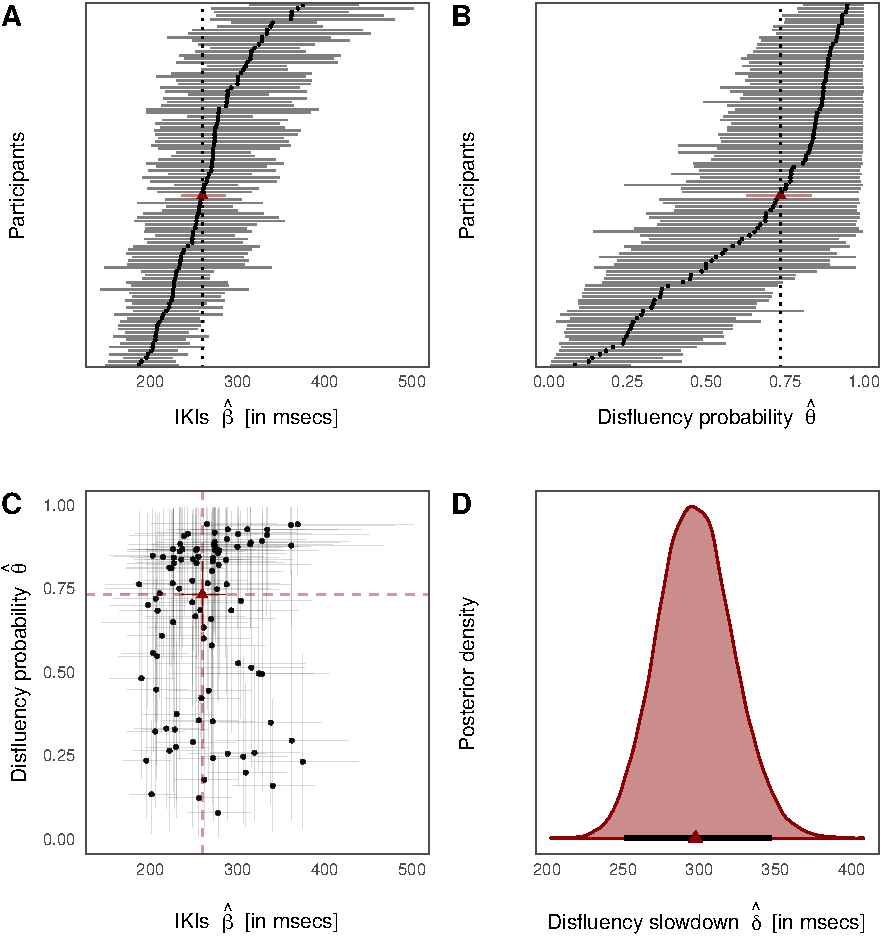
\includegraphics{report_files/figure-latex/parameters-1} 

}

\caption{By-participant parameter values for LF-bigrams and consonants task. Plot A and Plot B show the average IKIs for fluent typing and disfluency probabilities, respectively, for each participant (for a random subset of 75 participants for illustration); error bars indicate 95\% PIs, dotted vertical line shows the population estimate. Plot C--E show correlations (red line) between by-participant mean-posterior estimates of the consonants task and the LF-bigrams task for fluent typing (C), the autoregressor (D), and the disfluency probability (E).}\label{fig:parameters}
\end{figure}
\end{landscape}

Figure \ref{fig:parameters}C-E show between LF bigrams and consonants correlations for the by-participant estimates of the fluent-typing interval duration (C), the autocorrelation between subsequent keystroke intervals (D), and the disfluency probability. The correlations show that individuals with longer keystroke intervals for the LF-bigrams task also show longer keystroke intervals in the consonants task (Figure \ref{fig:parameters}C); a similar relationship can be seen for autoregression although in the consonants task participants generally show faster keystroke intervals across bigrams while for the LF bigrams task some participants speedup and other slowdown (Figure \ref{fig:parameters}D). No such correlation was found for the disfluency probability (Figure \ref{fig:parameters}E). Participants that exhibit many disfluencies in the consonants task do not necessarily show more disfluencies in the LF-bigrams task. In other words, the model parameters do not just capture individual differences but also task-specific differences with regards to typing speed and pausing behaviour.

Faster participants might, in principle, show larger disfluency magnitudes; i.e.~the size of the disfluency magnitude may vary by participant. To test this possibility we also implemented two models that are largely identical to model M3 (see equation \ref{eq:mog}): first, we allowed both the disfluency probability \(\theta\) and the disfluency magnitude \(\delta\) to vary by participant; second, \(\delta\) but not \(\theta\) was allowed to vary by participant. We compared the predictive performance of either model to model M3. Neither model was convincingly better than model M3, neither for the consonants task nor for the LF-bigrams task. For the consonants data, allowing \(\delta\) and \(\theta\) to vary by participant resulted in negligibly better predictive performance compared to model M3 (\(\Delta\widehat{elpd}\)=7, SE=4); holding the disfluency probability \(\theta\) constant while allowing the disfluency magnitude \(\delta\) to vary by participant revealed a lower predictive performance (\(\Delta\widehat{elpd}\)=-100, SE=50). The same patterns was found for LF bigrams: allowing \(\delta\) to vary rendered no predictive gain (\(\Delta\widehat{elpd}\)=-1, SE=0.50); fixing \(\theta\) and allowing \(\delta\) to vary showed a decrease in predictive performance (\(\Delta\widehat{elpd}\)=-30, SE=8). This comparison suggests that it is not the magnitude of the disfluencies (\(\delta\)) that varies across participants but the disfluency probability (mixing proportion \(\theta\)).

Overall, the values of the three process-central model parameters -- fluent typing speed, disfluency probability, and slowdown magnitude for disfluencies -- were found to be task sensitive. The LF-bigrams task shows shorter typing intervals, a lower disfluency probability compared to the consonants task and a shorter slowdown magnitude for typing disfluencies. Individual typing style was characterized by random variation in typing speed and in the probability but not in the magnitude of process disfluencies.

\hypertarget{discussion}{%
\section{Discussion}\label{discussion}}

Our aim was to provide a statistical model that allows to account for process disfluencies in keyboard-typing data. To address this aim we tested a series of Bayesian models on a lexical and a non-lexical copy-typing task. Model comparisons revealed that finite mixture models provided a better fit to inter-keystroke intervals of both copy-tasks compared to standard linear mixed-effects models. In other words, we showed that, among the models tested, data from copy-typing can be modelled best as a combination of fluent and disfluent typing intervals by means of an unknown individual mixing weight. We demonstrated how the model posterior can be used to infer estimates for three typing characteristics for individual participants and on the population level.

The best fitting model summarizes the typing process as a function of three process-relevant parameter values. Those are: (1) the population-level and by-participant keystroke transitions for fluent typing after accounting for process disfluencies; (2) population-level and by-participant mixing proportions indicating the probability of disfluent keystroke transitions; (3) the population-level disfluency magnitude, i.e.~slowdown in keystroke transitions. These parameter estimates are interesting for two reasons: first, they allow us to characterize the writing task at hand as a mixture of fluent and disfluent keystroke transitions as represented in Figure \ref{fig:modelv2}\footnote{This model is just one possibility of how the mixture-model parameters map onto copy-typing. Disfluencies might as well arise on a lower level, for example, when the typist is struggling to find the correct key}; second, by-participant parameter estimates allow us to extract characteristics for individual typists. On the basis of the population-level and individual parameter estimates, we can determine whether an individual is a fast / slow typist or has unusually high / low probability to exhibit disfluencies compared to the population estimates. Thus, the model can be used diagnostically to identify participants with larger disfluency probabilities or to compare pausing across groups of participants.

\begin{figure}[bp!]

{\centering 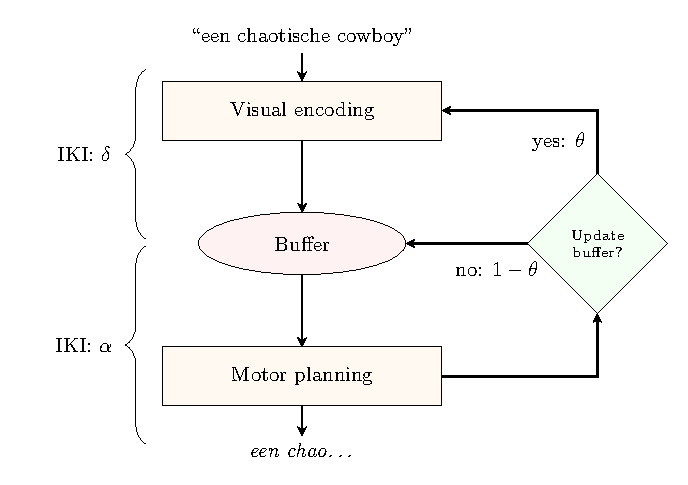
\includegraphics{spelling_decision_probs} 

}

\caption{Basic model of copy typing with mixture-model parameters. Disfluencies are the sum of $\alpha$ and $\delta$, where $\delta$ is the additional time that results from updating the letters buffered for motor encoding. The probability of disfluencies is indicated as $\theta$ mapping onto looks to the target string.}\label{fig:modelv2}
\end{figure}

The strength of this model is that it allows us to characterize the writing process and detect disfluencies in a principled way in line with what we know about keyboard typing. In particular, keyboard typing can be thought of as a process in which information cascades from higher to lower levels of activation; process inhibition on higher levels causes lags downstream. We have captured this process by characterizing the typing process as a mixture of fluent and disfluent keystroke transitions. Typing speed and the proportion of disfluent transitions depend on each typist's copying style. This is important because not distinguishing between between fluent and disfluent keystroke transitions can lead to incorrect inference about fluent typing. For example, collapsing across fluent and disfluent transitions might lead to the conclusion that task-related difficulty impacts on the execution of keystrokes even though the overall increased keystroke-transition duration was in fact the results of more frequent and longer pauses while typing speed itself may remain constant. From the present analysis we know that merely one-quarter of the data from the consonants task and two-thirds of the data from the LF-bigrams task were found to correspond to fluent keystroke transitions. Even after accounting for disfluent keystroke transitions, fluent typing was found to be two times slower in the consonants task compared to the LF-bigrams task. Not accounting for task-specific disfluency probabilities would result in biased estimates and, therefore, affect conclusions about task-related difference in typing speed.

Our results suggest that the probability and size of disfluencies are sensitive to task related factors. In the consonants task, disfluencies are indeed more probable than fluent transitions. This was not the case in the LF-bigrams task. Across participants the probability of typing disfluencies was relatively homogeneous in the LF-bigrams task but showed a larger variability in the consonants task. Similarly the average by-participant typing speed was more diverse in the consonants task compared to the LF-bigrams task. This contrast might be the result of a larger range of strategies that participants applied to copy consonant sequences than when copying the word triplet in the LF-bigrams task. For example, participants may have used \emph{n}-grams (one letter at a time or more) or spaces to chunk consonants before generating motor codes; in the lexical LF-bigrams task, word(s) or the entire phrase are better candidates for chunking than individual letters.

The variability in typing strategies across the sample may be understood as a function of typing skills and cognitive factors. For example, non-touch typists depend on memory resources to correctly copy the target string. This is because participants with poor typing skills have to shift gaze between keyboard and text more often than touch typists. Consequently, memory resources are more important for poor typists such that participants with a shorter memory span might update their memory representation of the target string more frequently than participants with a long memory span expressed as an increased disfluency probability. This might be less important for the typing performance of touch typists to the extent that touch typists have less need to search for keys corresponding to target letters. In contrast, the lower variability found for the LF-bigrams task can be understood as a more uniform use of copy-typing strategies across participants. Copy-typing strategies might have been more consistent for the LF-bigrams task because participants, especially those with poor typing skills, can make use existing knowledge (e.g.~lexical meaning of words, motor codes for bigrams) to relief memory demands. This is not possible for the consonants task. However, our results did not support a trade-off between typing speed and disfluency probability. This might be because disfluencies are not merely the result of a memory-representation update but are also related to difficulty finding the correct key and individual memory-span differences. Therefore the disfluency probability can be understood as an estimate for all non-typing related activities. As such the disfluency probability may be an indicator of memory span (Grabowski et al., 2010; Olive, 2014), low level reading skill (De Smet et al., 2018) and individual typing skills.

The central advantage of using mixture models to account for typing disfluencies is that we can by-pass threshold values to define disfluencies and include it as individual typing-skill property in the analysis of writing-process data. Mixture models provide estimates for fluent typing while accounting for disfluencies by modelling fluent and disfluent typing as a mixture process. At the same time, mixture models provide disfluency estimates as expression for individual and task-specific typing difficulty. It is impossible to know the upper bound for fluent and the lower bound for disfluent transitions from screening keystroke data. Using threshold values ignores that some participants are generally slower typists and some tasks are more difficult. Mixture models allow us to capture disfluencies as a latent process in a principled manner. This is important because disfluencies must be understood as relative to an individuals' typing speed given the task at hand (Wengelin, 2006). Therefore, mixture models allow us to test predictions about typing disfluencies in certain populations such as learning typists, L2 typists and individuals with genuine typing difficulty after account for individual differences in typing speed or vice versa. For example, some individuals that might be classified as having typing problems might not have excessive numbers of pauses but merely longer key transitions, while normal typists use pauses to prepare larger linguistic units. In other words, the presented model can be used to test hypotheses about psychological factors (e.g.~memory demands, writing experience, proficiency in writing in a second language) that might affect the ratio of disfluencies in the writing process. If disfluencies are crucial to identify poor typists in a sample, mixture models might be used as diagnostic tool. Also, mixture models allow us to directly test whether the number of disfluencies can be changed as response to an keyboard typing intervention. As an avenue for future research, mixture models as presented in this paper can be used for different types of writing tasks and particular populations.

Writing involves processing on various levels of mental representation. As activation cascades from higher to lower levels of representation, a delay on any of these levels causes disfluencies. While we modelled this process as a binary distinction between fluent and disfluent typing, processing difficulty on different levels might be associated with different disfluency magnitudes and might be cumulative. If the size of the disfluency is assumed to depend on the inhibited process upstream or combination of processes, this can be implemented as additional mixture component(s) (similar to Baaijen et al., 2012; see also Almond et al., 2012) to address different types of disfluencies (Medimorec et al., 2017; Medimorec \& Risko, 2016; Wengelin, 2001). In other words extensions of mixture models allow us to test different hypotheses about the cascade of processes involved in writing and language production.

\hypertarget{references}{%
\section{References}\label{references}}

\begingroup
\setlength{\parindent}{-0.5in}
\setlength{\leftskip}{0.5in}

\hypertarget{ref}{}

\endgroup

\hypertarget{refs}{}
\begin{cslreferences}
\leavevmode\hypertarget{ref-almond2012preliminary}{}%
Almond, R., Deane, P., Quinlan, T., Wagner, M., \& Sydorenko, T. (2012). \emph{A preliminary analysis of keystroke log data from a timed writing task} (Research Report No. RR-12-23). Educational Testing Service.

\leavevmode\hypertarget{ref-alves2015progress}{}%
Alves, R. A., \& Limpo, T. (2015). Progress in written language bursts, pauses, transcription, and written composition across schooling. \emph{Scientific Studies of Reading}, \emph{19}(5), 374--391.

\leavevmode\hypertarget{ref-baaijen2018discovery}{}%
Baaijen, V. M., \& Galbraith, D. (2018). Discovery through writing: Relationships with writing processes and text quality. \emph{Cognition and Instruction}, \emph{36}(3), 199--223.

\leavevmode\hypertarget{ref-baaijen2012keystroke}{}%
Baaijen, V. M., Galbraith, D., \& de Glopper, K. (2012). Keystroke analysis: Reflections on procedures and measures. \emph{Written Communication}, \emph{29}(3), 246--277.

\leavevmode\hypertarget{ref-baa08book}{}%
Baayen, R. H. (2008). \emph{Analyzing linguistic data. A practical introduction to statistics using R}. Cambridge University Press.

\leavevmode\hypertarget{ref-beers2017effects}{}%
Beers, S. F., Mickail, T., Abbott, R., \& Berninger, V. (2017). Effects of transcription ability and transcription mode on translation: Evidence from written compositions, language bursts and pauses when students in grades 4 to 9, with and without persisting dyslexia or dysgraphia, compose by pen or by keyboard. \emph{Journal of Writing Research}, \emph{9}(1), 1--25.

\leavevmode\hypertarget{ref-bock2014syntactically}{}%
Bock, J. K., \& Ferreira, V. S. (2014). Syntactically speaking. In M. Goldrick, V. S. Ferreira, \& M. Miozzo (Eds.), \emph{The Oxford Handbook of Language Production} (pp. 21--46). Oxford University Press.

\leavevmode\hypertarget{ref-carpenter2016stan}{}%
Carpenter, B., Gelman, A., Hoffman, M. D., Lee, D., Goodrich, B., Betancourt, M., Brubaker, M. A., Guo, J., Li, P., \& Riddell, A. (2016). Stan: A probabilistic programming language. \emph{Journal of Statistical Software}, \emph{20}.

\leavevmode\hypertarget{ref-chanquoy1996writing}{}%
Chanquoy, L., Foulin, J.-N., \& Fayol, M. (1996). Writing in adults: A real-time approach. In G. Rijlaarsdam, H. Van den Bergh, \& M. Couzijn (Eds.), \emph{Theories, models and methodology in writing research} (pp. 36--44). Amsterdam University Press.

\leavevmode\hypertarget{ref-christiansen2016now}{}%
Christiansen, M. H., \& Chater, N. (2016). The now-or-never bottleneck: A fundamental constraint on language. \emph{Behavioral and Brain Sciences}, \emph{39}, 1--72. \url{https://doi.org/\%20http://dx.doi.org/10.1017/S0140525X1500031X}

\leavevmode\hypertarget{ref-chukharev2019combined}{}%
Chukharev-Hudilainen, E., Saricaoglu, A., Torrance, M., \& Feng, H.-H. (2019). Combined deployable keystroke logging and eyetracking for investigating L2 writing fluency. \emph{Studies in Second Language Acquisition}, \emph{41}(3), 583--604.

\leavevmode\hypertarget{ref-chukharev2014pauses}{}%
Chukharev-Khudilaynen, E. (2014). Pauses in spontaneous written communication: A keystroke logging study. \emph{Journal of Writing Research}, \emph{6}(1), 61--84.

\leavevmode\hypertarget{ref-conijn2019understanding}{}%
Conijn, R., Roeser, J., \& van Zaanen, M. (2019). Understanding the keystroke log: The effect of writing task on keystroke features. \emph{Reading and Writing}, \emph{32}(9), 2353--2374.

\leavevmode\hypertarget{ref-conijn2019typo}{}%
Conijn, R., Van Zaanen, M., Leijten, M., \& Van Waes, L. (2019). How to typo? Building a process-based model of typographic error revisions. \emph{The Journal of Writing Analytics}, \emph{3}, 69--95.

\leavevmode\hypertarget{ref-connelly2012predicting}{}%
Connelly, V., Dockrell, J. E., Walter, K., \& Critten, S. (2012). Predicting the quality of composition and written language bursts from oral language, spelling, and handwriting skills in children with and without specific language impairment. \emph{Written Communication}, \emph{29}(3), 278--302.

\leavevmode\hypertarget{ref-de2018exploring}{}%
De Smet, M. J. R., Leijten, M., \& Van Waes, L. (2018). Exploring the process of reading during writing using eye tracking and keystroke logging. \emph{Written Communication}, \emph{35}(4), 411--447.

\leavevmode\hypertarget{ref-eltahir2004dynamic}{}%
Eltahir, W. E., Salami, M. J. E., Ismail, A. F., \& Lai, W. K. (2004). Dynamic keystroke analysis using AR model. \emph{IEEE International Conference on Industrial Technology}, \emph{3}, 1555--1560.

\leavevmode\hypertarget{ref-farrell2018computational}{}%
Farrell, S., \& Lewandowsky, S. (2018). \emph{Computational modeling of cognition and behavior}. Cambridge University Press.

\leavevmode\hypertarget{ref-feldman2019lexical}{}%
Feldman, L. B., Dale, R., \& van Rij, J. (2019). Lexical and frequency effects on keystroke timing: Challenges to a lexical search account from a type-to-copy task. \emph{Frontiers in Communication}, \emph{4}, 17.

\leavevmode\hypertarget{ref-gelman2006prior}{}%
Gelman, A. (2006). Prior distributions for variance parameters in hierarchical models (comment on article by Browne and Draper). \emph{Bayesian Analysis}, \emph{1}(3), 515--533.

\leavevmode\hypertarget{ref-gelman2014}{}%
Gelman, A., Carlin, J. B., Stern, H. S., Dunson, D. B., Vehtari, A., \& Rubin, D. B. (2014). \emph{Bayesian data analysis} (3rd ed.). Chapman; Hall/CRC.

\leavevmode\hypertarget{ref-gelman1992}{}%
Gelman, A., \& Rubin, D. B. (1992). Inference from iterative simulation using multiple sequences. \emph{Statistical Science}, \emph{7}(4), 457--472.

\leavevmode\hypertarget{ref-grabowski2008internal}{}%
Grabowski, J. (2008). The internal structure of university students' keyboard skills. \emph{Journal of Writing Research}, \emph{1}(1).

\leavevmode\hypertarget{ref-grabowski2010second}{}%
Grabowski, J., Weinzierl, C., \& Schmitt, M. (2010). Second and fourth graders' copying ability: From graphical to linguistic processing. \emph{Journal of Research in Reading}, \emph{33}(1), 39--53.

\leavevmode\hypertarget{ref-guo2018modeling}{}%
Guo, H., Deane, P. D., van Rijn, P. W., Zhang, M., \& Bennett, R. E. (2018). Modeling basic writing processes from keystroke logs. \emph{Journal of Educational Measurement}, \emph{55}(2), 194--216.

\leavevmode\hypertarget{ref-hayes2012evidence}{}%
Hayes, J. R. (2012). Evidence from language bursts, revision, and transcription for translation and its relation to other writing processes. In M. Fayol, D. Alamargot, \& V. Berninger (Eds.), \emph{Translation of thought to written text while composing} (pp. 15--25). Psychology Press.

\leavevmode\hypertarget{ref-hoaglin1987fine}{}%
Hoaglin, D. C., \& Iglewicz, B. (1987). Fine-tuning some resistant rules for outlier labeling. \emph{Journal of the American Statistical Association}, \emph{82}(400), 1147--1149.

\leavevmode\hypertarget{ref-hoffman2014no}{}%
Hoffman, M. D., \& Gelman, A. (2014). The No-U-Turn sampler: Adaptively setting path lengths in Hamiltonian Monte Carlo. \emph{Journal of Machine Learning Research}, \emph{15}(1), 1593--1623.

\leavevmode\hypertarget{ref-jefferys1992ockham}{}%
Jefferys, W. H., \& Berger, J. O. (1992). Ockham's razor and Bayesian analysis. \emph{American Scientist}, \emph{80}(1), 64--72.

\leavevmode\hypertarget{ref-kaufer1986composing}{}%
Kaufer, D. S., Hayes, J. R., \& Flower, L. (1986). Composing written sentences. \emph{Research in the Teaching of English}, \emph{20}(2), 121--140.

\leavevmode\hypertarget{ref-lambert2018student}{}%
Lambert, B. (2018). \emph{A student's guide to Bayesian statistics}. Sage.

\leavevmode\hypertarget{ref-lee2014bayesian}{}%
Lee, M. D., \& Wagenmakers, E.-J. (2014). \emph{Bayesian cognitive modeling: A practical course}. Cambridge University Press.

\leavevmode\hypertarget{ref-leijten2011coordinating}{}%
Leijten, M., De Maeyer, S., \& Van Waes, L. (2011). Coordinating sentence composition with error correction: A multilevel analysis. \emph{Journal of Writing Research}, \emph{2}(3), 331--363.

\leavevmode\hypertarget{ref-leijten2013keystroke}{}%
Leijten, M., \& Van Waes, L. (2013). Keystroke logging in writing research: Using Inputlog to analyze and visualize writing processes. \emph{Written Communication}, \emph{30}(3), 358--392.

\leavevmode\hypertarget{ref-logan2011hierarchical}{}%
Logan, G. D., \& Crump, M. J. C. (2011). Hierarchical control of cognitive processes: The case for skilled typewriting. In B. Ross (Ed.), \emph{Psychology of learning and motivation} (Vol. 54, pp. 1--27). Academic Press.

\leavevmode\hypertarget{ref-mcelreath2016statistical}{}%
McElreath, R. (2016). \emph{Statistical rethinking: A Bayesian course with examples in R and Stan}. CRC Press.

\leavevmode\hypertarget{ref-medimorec2016effects}{}%
Medimorec, S., \& Risko, E. F. (2016). Effects of disfluency in writing. \emph{British Journal of Psychology}, \emph{107}(4), 625--650.

\leavevmode\hypertarget{ref-medimorec2017disfluency}{}%
Medimorec, S., Young, T. P., \& Risko, E. F. (2017). Disfluency effects on lexical selection. \emph{Cognition}, \emph{158}, 28--32.

\leavevmode\hypertarget{ref-not05}{}%
Nottbusch, G., Grimm, A., Weingarten, R., \& Will, U. (2005). Syllabic sructures in typing: Evidence from deaf writers. \emph{Reading \& Writing}, \emph{18}(6), 497--526.

\leavevmode\hypertarget{ref-olive2014toward}{}%
Olive, T. (2014). Toward a parallel and cascading model of the writing system: A review of research on writing processes coordination. \emph{Journal of Writing Research}, \emph{6}(2), 173--194.

\leavevmode\hypertarget{ref-papaspiliopoulos2007general}{}%
Papaspiliopoulos, O., Roberts, G. O., \& Sköld, M. (2007). A general framework for the parametrization of hierarchical models. \emph{Statistical Science}, \emph{22}(1), 59--73.

\leavevmode\hypertarget{ref-pinet2016typing}{}%
Pinet, S., Ziegler, J. C., \& Alario, F.-X. (2016). Typing is writing: Linguistic properties modulate typing execution. \emph{Psychonomic Bulletin \& Review}, \emph{23}(6), 1898--1906.

\leavevmode\hypertarget{ref-quene2004multi}{}%
Quené, H., \& Van den Bergh, H. (2004). On multi-level modeling of data from repeated measures designs: A tutorial. \emph{Speech Communication}, \emph{43}(1-2), 103--121.

\leavevmode\hypertarget{ref-roeser2019advance}{}%
Roeser, J., Torrance, M., \& Baguley, T. (2019). Advance planning in written and spoken sentence production. \emph{Journal of Experimental Psychology: Learning, Memory, and Cognition}, \emph{45}(11), 1983--2009.

\leavevmode\hypertarget{ref-sah08}{}%
Sahel, S., Nottbusch, G., Grimm, A., \& Weingarten, R. (2008). Written production of german compounds: Effects of lexical frequency and semantic transparency. \emph{Written Language \& Literacy}, \emph{11}(2), 211--228.

\leavevmode\hypertarget{ref-salthouse1984effects}{}%
Salthouse, T. A. (1984). Effects of age and skill in typing. \emph{Journal of Experimental Psychology: General}, \emph{113}(3), 345--371.

\leavevmode\hypertarget{ref-schoner2002timing}{}%
Schöner, G. (2002). Timing, clocks, and dynamical systems. \emph{Brain and Cognition}, \emph{48}(1), 31--51.

\leavevmode\hypertarget{ref-rstan}{}%
Stan Development Team. (2015a). \emph{Stan: A C++ library for probability and sampling}. \url{http://mc-stan.org/}.

\leavevmode\hypertarget{ref-rstan2}{}%
Stan Development Team. (2015b). \emph{Stan modeling language user's guide and reference manual}. \url{http://mc-stan.org/}.

\leavevmode\hypertarget{ref-sullivan2002self}{}%
Sullivan, K. P. H., \& Lindgren, E. (2002). Self-assessment in autonomous computer-aided second language writing. \emph{ELT Journal}, \emph{56}(3), 258--266.

\leavevmode\hypertarget{ref-torrance2016adolescent}{}%
Torrance, M., Rønneberg, V., Johansson, C., \& Uppstad, P. H. (2016). Adolescent weak decoders writing in a shallow orthography: Process and product. \emph{Scientific Studies of Reading}, \emph{20}(5), 375--388.

\leavevmode\hypertarget{ref-van1991handwriting}{}%
Van Galen, G. P. (1991). Handwriting: Issues for a psychomotor theory. \emph{Human Movement Science}, \emph{10}(2), 165--191.

\leavevmode\hypertarget{ref-van2015fluency}{}%
Van Waes, L., \& Leijten, M. (2015). Fluency in writing: A multidimensional perspective on writing fluency applied to L1 and L2. \emph{Computers and Composition}, \emph{38}, 79--95.

\leavevmode\hypertarget{ref-van2016keystroke}{}%
Van Waes, L., Leijten, M., Lindgren, E., \& Wengelin, Å. (2016). \emph{Keystroke logging in writing research: Analyzing online writing processes}. 410--426.

\leavevmode\hypertarget{ref-van2019multilingual}{}%
Van Waes, L., Leijten, M., Pauwaert, T., \& Van Horenbeeck, E. (2019). A multilingual copy task: Measuring typing and motor skills in writing with inputlog. \emph{Journal of Open Research Software}, \emph{7}(30), 1--8.

\leavevmode\hypertarget{ref-van2010reading}{}%
Van Waes, L., Leijten, M., \& Quinlan, T. (2010). Reading during sentence composing and error correction: A multilevel analysis of the influences of task complexity. \emph{Reading and Writing}, \emph{23}(7), 803--834. \url{https://doi.org/10.1007/s11145-009-9190-x}

\leavevmode\hypertarget{ref-waes2019}{}%
Van Waes, L., Leijten, M., Roeser, J., Olive, T., \& Grabowski, J. (2020). Designing a copy task to measure typing and motor skills in writing research. \emph{Journal of Writing Research}.

\leavevmode\hypertarget{ref-vasishth2017}{}%
Vasishth, S., Chopin, N., Ryder, R., \& Nicenboim, B. (2017). Modelling dependency completion in sentence comprehension as a Bayesian hierarchical mixture process: A case study involving Chinese relative clauses. \emph{ArXiv E-Prints}.

\leavevmode\hypertarget{ref-vasishth2017feature}{}%
Vasishth, S., Jäger, L. A., \& Nicenboim, B. (2017). Feature overwriting as a finite mixture process: Evidence from comprehension data. \emph{arXiv Preprint arXiv:1703.04081}.

\leavevmode\hypertarget{ref-vehtari2015pareto}{}%
Vehtari, A., Gelman, A., \& Gabry, J. (2015). Pareto smoothed importance sampling. \emph{arXiv Preprint arXiv:1507.02646}.

\leavevmode\hypertarget{ref-vehtari2017practical}{}%
Vehtari, A., Gelman, A., \& Gabry, J. (2017). Practical Bayesian model evaluation using leave-one-out cross-validation and WAIC. \emph{Statistics and Computing}, \emph{27}(5), 1413--1432.

\leavevmode\hypertarget{ref-wagenmakers2007linear}{}%
Wagenmakers, E.-J., \& Brown, S. (2007). On the linear relation between the mean and the standard deviation of a response time distribution. \emph{Psychological Review}, \emph{114}(3), 830--841. \url{https://doi.org/10.1037/0033-295X.114.3.830}

\leavevmode\hypertarget{ref-wallot2013typewriting}{}%
Wallot, S., \& Grabowski, J. (2013). Typewriting dynamics: What distinguishes simple from complex writing tasks? \emph{Ecological Psychology}, \emph{25}(3), 267--280.

\leavevmode\hypertarget{ref-wengelin2001disfluencies}{}%
Wengelin, Å. (2001). Disfluencies in writing -- Are they like in speaking? \emph{ISCA Tutorial and Research Workshop (ITRW) on Disfluency in Spontaneous Speech}.

\leavevmode\hypertarget{ref-wen02}{}%
Wengelin, Å. (2002). \emph{Text production in adults with reading and writing difficulties} {[}PhD thesis{]}. Göteborg University.

\leavevmode\hypertarget{ref-wen06}{}%
Wengelin, Å. (2006). Examining pauses in writing: Theory, methods and empirical data. In K. P. H. Sullivan \& E. Lindgren (Eds.), \emph{Computer keystroke logging and writing: Methods and applications} (Vol. 18, pp. 107--130). Elsevier.

\leavevmode\hypertarget{ref-wing1973response}{}%
Wing, A. M., \& Kristofferson, A. B. (1973). Response delays and the timing of discrete motor responses. \emph{Perception \& Psychophysics}, \emph{14}(1), 5--12.

\leavevmode\hypertarget{ref-yamaguchi2014pushing}{}%
Yamaguchi, M., \& Logan, G. D. (2014). Pushing typists back on the learning curve: Revealing chunking in skilled typewriting. \emph{Journal of Experimental Psychology: Human Perception and Performance}, \emph{40}(2), 592--612.

\leavevmode\hypertarget{ref-zhang2019there}{}%
Zhang, M., Bennett, R. E., Deane, P., \& Rijn, P. W. van. (2019). Are there gender differences in how students write their essays? An analysis of writing processes. \emph{Educational Measurement: Issues and Practice}, \emph{38}(2), 14--26.
\end{cslreferences}

\end{document}
